\documentclass{article}

\usepackage[utf8x]{inputenc}
\usepackage{amssymb}
\usepackage{amsthm}
\usepackage{amsmath}
\usepackage{algorithm}
\usepackage{algpseudocode}
\usepackage{color}
\usepackage{multicol}
\usepackage{tikz}
\usetikzlibrary{automata, positioning, chains,fit,shapes}
\definecolor{keywordcolor}{rgb}{0.7, 0.1, 0.1}   % red
\definecolor{commentcolor}{rgb}{0.4, 0.4, 0.4}   % grey
\definecolor{symbolcolor}{rgb}{0.0, 0.1, 0.6}    % blue
\definecolor{sortcolor}{rgb}{0.1, 0.5, 0.1}      % green
\usepackage{listings}
\def\lstlanguagefiles{lstlean.tex}
\lstset{
    language=lean,
    xleftmargin=-6em
}

\newtheorem{example}{Example}
\newtheorem{theorem}{Theorem}
\newtheorem{lemma}{Lemma}



\title{LEAN-aided verification of datalog reasoning results}
\author{Johannes Tantow}

\begin{document}
    \maketitle
    \section{Introduction}
    \section{Preliminaries}
    \subsection{Datalog}
        Syntactically datalog bears many similarities to first-order logic and may be viewed as a fragment of it, but the semantics are more specialized. In order to define the syntax we will introduce some definitions from first-order logic.

        Firstly, we consider in general three countably infinite sets $R$, that consists of relation symbols, $C$, that consists of constants, and $V$, that consists of variables. In order to differentiate between constants and variables we require that $V \cap C  = \emptyset$. Each relation symbol has an associated arity $ar: R \to \mathbb{N}$. As we will only consider finite programs and databases, there will always be at most finitely many relation symbols, constants or variables in usage, but by requiring these sets to be countably infinite we make sure that we always have a sufficient amount. 
        
        A \textit{term} is either a constant or variable. In contrast to first-order logic or logic programming, we do not allow function symbols in datalog, but there are extensions of datalog that allow using some function symbols like addition or multiplication as terms as well.

        An \textit{atom} is of the form $A(t_1, ..., t_{ar(A)})$ where $A$ is a relation symbol and $t_1,..., t_{ar(A)}$ are terms. The atom variables of $A(t_1, ..., t_{ar(A)})$ are the set of those $t_i$ which are variables. A \textit{ground atom} is an atom where the atom variables are the empty set, i.e. every term is a constant.
        
        A \textit{rule} is a expression of the form $H \leftarrow B_1 \land ... \land B_n$, where $H$ and all $B_i$ are atoms. $H$ is called the head of the rule and $\{B_1,.., B_n\}$ is the body of the rule. If $H$ and all $B_i$ are ground atoms, then we call this rule a \textit{ground rule}. If the body is empty, we call a rule a \textit{fact}. A rule is called \textit{safe}, if every variables in the atom variables of the head is also in the atom variables of some atom in the body. 

        A \textit{program} is a finite set of rules. The program is safe, if all its rules are.

        A datalog engine calculates the semantics of a datalog program, which we will define shortly. The non-fact rules of program are often general rules that can be used in many contexts, whereas the facts encode a specific context. In order to reuse programs, the facts are often outsourced in database, which we can imagine as a set of ground atoms. In the semantics we assume that these facts are then added back to the program for easier definitions.

        Datalog has three major semantics: model-theoretic, proof theoretic and fixed-point based. These three semantics coincide. The semantics of a datalog program $P = \{r_1,...,r_k\}$ is a set of ground atoms.

        For the model-theoretic semantics we describe the semantics as a specific model of the program. So far $P$ might however contain variables, which have to be mapped to something. Therefore we first transform $P$ into the \textit{ground program}, $ground(P)$. For this we consider \textit{groundings} or \textit{instantiations}, which are functions from $V$ to $C$. We can apply a grounding $g$ to an atom $a$ to aquire a ground atom by replacing a variable $v$ with $g(v)$. We may write this also as $g(a)$ and can apply grounding to a rule $r$ as well by applying it to every atom in the body and the head, which we denote as $g(r)$. The ground program is then defined as $ground(P) = \{r' \mid \exists r \in P. \exists g. g(r) = r' \}$

        A set of ground atoms $I$ (\textit{interpretation}) is a \textit{model} of a ground rule $r$, if whenever the body of $r$ is a subset of $I$ also the head appears inside $I$. An interpretation is a model of a ground program $P$ if it is all model for all ground rules in $P$.

        We would like to define the model-theoretic semantics of $P$ as the model of $ground(P)$. In general there are however multiple models of $ground(P)$, so that this would not be unambiguous. It might contain ground atoms without a ground rule having this atom as a head. It can however be proven that there always exists a minimal model of $ground(P)$. We define this as the model-theoretic semantics of $P$

        A different view is to look why an atom $a$ is inside the minimal model. It might be because there was a ground rule in $ground(P)$ of which $a$ is the head and for which the body is already in the minimal model. Now we can again ask this for all elements in the body until we reach facts, which have to be true. This can be seen as a proof for $a$. This proof can be modelled as a rooted tree which nodes are ground atoms. A tree is a \textit{valid proof tree} for $a$ in $P$ if the following conditions hold.
        \begin{enumerate}
            \item The root is $a$
            \item For each leaf exists a fact in $ground(P)$
            \item For each node $n$ and its predecessors $m_1,..., m_k$ exists a rule in $ground(P)$ which the head $n$ and the body $\{ m_1,..., m_k\}$
        \end{enumerate}
        The proof-theoretic semantics is then the set of ground atoms for which a valid proof tree in $P$ exists.

        The previous two semantics both provide clear definitions, but do not tell us how to arrive at this set. The fixed point semantics offers way to do this. For this we consider the following operator, that takes a set of ground atoms as an input.
        
        \[T_P(I) = \{a \mid \exists r \in ground(P), head(r) = a \land body(r) \subseteq I\}\]

        This operator can be proven to be monotonic and therefore a least fixed-point exists by the Knaster-Tarski theorem exists. It can be computed by starting with $\emptyset$ for $I$ and repeatedly apply $T_P$ until we find the fixed-point. This semantics is the basis for the practical implementations of datalog engines.

        All three semantics can be proven to be equivalent, which we will do later in Lean for the proof-theoretic and model-theoretic semantics.

        Additionally, it turns out that every non-safe program can be transformed into a safe program by introducing new relation symbols, such that for all original relation symbols the semantics coincide.
    \section{Datalog in Lean}
        
        We introduced Datalog in the previous chapter. Here we show our implementation in Lean that we will use later to show the correctness of our algorithms.

        We started defining datalog using sets for constants, variables and relation symbols. In order to have a more compact representation we use the idea of a signature, that stores all these informations.

        \begin{lstlisting}
            structure signature where
                (constants: Type)
                (vars: Type)
                (relationSymbols: Type)
                (relationArity: relationSymbols → ℕ)
        \end{lstlisting}

        We no longer require that the constants and variables are distinct sets as the constructor for terms allows us to identify the type of a term. We will continue to define the other syntactic elements of datalog. The signature unless displayed otherwise will be $\tau$.

        \begin{lstlisting}
            inductive term :
            | constant : τ.constants → term τ
            | variableDL : τ.vars → term τ
            deriving DecidableEq
        \end{lstlisting}

        As we want to use these objects in practical algorithms we need a way to see if two terms are the same to e.g. replace a variable by a constant. We use Leans ability to automatically create a decidable function for equality for our inductive types and structure from the given functions for the equality of the types from the signature. This allows us to use statements like \texttt{a = b} for atoms \texttt{a, b} in the program we describe in the later sections.
    
        For atoms we have to make sure that the amount of terms matches the arity of the relation symbol. Therefore the structure has an additonal element that is a proof of this property. Two atoms are equal if all fields in the structure are equal. Since propositions as this proof are always equal, it is enough to show that the terms and the symbols are equal.

        \begin{lstlisting}
            structure atom where
                (symbol: τ.relationSymbols)
                (atom_terms: List (term τ ))
                (term_length: atom_terms.length = τ.relationArity symbol)
            deriving DecidableEq

            lemma atomEquality (a1 a2: atom τ): 
            a1 = a2 ↔ a1.symbol = a2.symbol ∧ a1.atom_terms = a2.atom_terms 

        \end{lstlisting}

        Rules and programs can be expressed relatively straight forward. For programs we use \texttt{abbrev}, which introduces program as an alias for \texttt{Finset(rule $\tau$)} from \texttt{mathlib},  instead of defining a new type as this allows us to use the common set operations without the need to redefine them.

        \begin{lstlisting}
            structure rule where
                (head: atom τ)
                (body: List (atom τ))
                deriving DecidableEq

            abbrev program := Finset (rule τ)
        \end{lstlisting}

        We have previously introduced ground atoms as atoms whose terms are only constants. There are at least two options to represent them here. Firstly we could define a structure for ground atoms that extends atoms by a predicate that shows that there are only constants present. The second option is to define an entirely new structure similar to atoms but allow only constants instead of terms. The first options show directly that every ground atom is an atom which we would have to establish separatedly in the second option. The second option allows directly to define the functions on a list of constants instead of having to cast the list of terms of a ground atom directly to a list of constants and allows to use the complete induction schema when defining functions on ground atoms. The second option seemed to offer more advantegous and was therefore chosen.

        \begin{lstlisting}
            structure groundAtom  where
                symbol: τ.relationSymbols
                atom_terms: List (τ.constants )
                term_length: atom_terms.length = τ.relationArity symbol
            deriving DecidableEq
        \end{lstlisting}

        Now we need a function that maps \texttt{groundAtom} back to \texttt{atom}. For this we can map the \texttt{atom\_terms} list in \texttt{groundAtom} with \texttt{term.constant} to term. Additionally we need to show that the \texttt{term\_length} property is preserved. Luckily, this is already proven in mathlib.


        \begin{lstlisting}
            lemma listMapPreservesTermLength (ga: groundAtom τ): 
            (List.map term.constant ga.atom_terms).length = 
             τ.relationArity ga.symbol :=
            by
                rw [List.length_map]
                apply ga.term_length

            def groundAtom.toAtom (ga: groundAtom τ): atom τ:= 
            {
                symbol:=ga.symbol,
                atom_terms:= List.map term.constant ga.atom_terms,
                term_length:= listMapPreservesTermLength ga
            }
        \end{lstlisting}

        Additionally, we need later that two \texttt{groundAtom} are equal iff the result of \texttt{toAtom} is equal. Similarly, we can define ground rules and functions to convert them to rules.

        For now we have only seen 


        We formalize two semantics here. Firstly, we need the proof-theoretic semantics. Proof trees are a good way to show why an element must be in the solution and output already by multiple datalog engines. There is however to the best of our current knowledge no short certificate similar to proof trees to show the absence of elements. In order to show that a solution is complete we need another method. Both the fixed-point and the model-theoretic semantics offer help in this case. Both are the least element of some set (of fixed-point or of models respectively). Therefore it is enough to show that it is a member of this set for the other direction.

        For the semantics we need the concept of the database. We do not want to deal with the implementation details of a database. We consider it as a black box that returns for a ground atom whether it is in the database. It is a function that returns \texttt{Bool}, because we want computable databases.

        \begin{lstlisting}
            class database (τ: signature) 
            [DecidableEq τ.vars] [DecidableEq τ.relationSymbols]
            [DecidableEq τ.constants]:=
            (contains: groundAtom τ → Bool)
        \end{lstlisting}
        

        We start by defining the proof-theoretic semantics. For this we need to formalize trees. The tree is supposed to start from the facts and then expand upwards by the application of rules. As the body of rules is in general unbounded, we also require trees with an unbounded number of children, which we realize via lists.

        \begin{lstlisting}
            inductive tree (A: Type)
            | node: A → List (tree A) → tree A        
        \end{lstlisting}

        In contrast to binary trees, we will need to use functions for lists to define functions on trees. Most interesting function will however need a proof of termination due to this tree model. 
        
        \begin{lstlisting}
            def root: tree A → A
            | tree.node a _ => a

            def children: tree A → List (A)
            | tree.node _ l => List.map root l

            def listMax {A: Type} (f: A → ℕ): List A → ℕ
            | [] => 0
            | (hd::tl) => 
                if f hd > listMax f tl 
                then f hd 
                else listMax f tl

            def height: tree A → ℕ
            | tree.node a l => 
                1 + listMax (fun ⟨x, _h⟩ => height x) l.attach
            termination_by height t => sizeOf t
            decreasing_by
                simp_wf
                apply Nat.lt_trans (m:= sizeOf l)
                apply List.sizeOf_lt_of_mem _h
                simp
        \end{lstlisting}
        
        Height is recursively called on the elements of in the list via the listMax function. Lean can not identify that this terminates so we have to provide a proof of termination. This is done in Lean by providing a well-founded relation that takes part of the input and show that the recursive calls of the function are only on elements that are smaller in this relation. Due to the well-foundedness there are no infinite descending chains and the function must terminate.  We use the \texttt{sizeOf} function that is built in for any inductive type and maps an element to the sucessor of the sum of the \texttt{sizeOf} values of the elements used in the sucessor. If we show that this always decreases then the function will terminate as the natural numbers are well-founded.

        In contrast to just using the list, we call listMax on \texttt{List.attach} instead. \texttt{List.attach} takes a list $l$ and creates a new list consisting of pairs of the original elements and a proof that the element is in $l$. This proof can be later used when proving termination.

        We have to show a statement of the form $\mathtt{sizeOf} x < 1 + \mathtt{sizeOf} a + \mathtt{sizeOf} l$. We use the transitivity property of the linear order to show this via showing first that $\mathtt{sizeOf} x < \mathtt{sizeOf} l$ and secondly that $\mathtt{sizeOf} l < 1 + \mathtt{sizeOf} a + \mathtt{sizeOf} l$. This second statement is obviously true and can be found by \texttt{simp}. For the first statement we can use the fact that the size of a member of a list is smaller than the size of the list. Due to using \texttt{l.attach} we have a proof for this available and finish the proof.
        This way of proving termination is the standard way we use in this model and will be omitted for further tree functions.

        Proof trees are then trees that have \texttt{groundAtom} as it vertices and we can formulate the validness criteria. There are two cases. If we are at leaf, i.e. the list of children is empty, then we simply check the database. Else there must exist a rule $r$ from the program and a grounding $g$ so that applying $g$ to $r$ matches the rule created from the current node and its children. Additionally all child trees must be valid as well.

        \begin{lstlisting}
            abbrev proofTree' (τ: signature) := tree (groundAtom τ)

            def isValid(P: program τ) (d: database τ) (t: proofTree τ): 
            Prop :=
            match t with
            | proofTree.node a l => 
            ( ∃(r: rule τ) (g:grounding τ), 
                r ∈ P ∧ 
                ruleGrounding r g = groundRuleFromAtoms a (List.map root l)
                ∧ l.attach.All₂ (fun ⟨x, _h⟩ => isValid P d x)) 
            ∨ (l = [] ∧ d.contains a)
        \end{lstlisting}

        The proof-theoretic semantics is then simply the set of ground atoms that are the root of a valid proof tree.

        \begin{lstlisting}
            def proofTheoreticSemantics (P: program τ) (d: database τ): 
            interpretation τ:= 
            {a: groundAtom τ | ∃(t: proofTree τ), root t = a ∧ isValid P d t}
        \end{lstlisting}

        After that we define the model-theoretic semantics. We choose the model-theoretic semantics over the fixed points semantics as we can directly construct the model and do not have to show that a fixed-point exists. Checking them in practice seems to be similar. 

        An interpretation is a set of ground atoms, that may be a model. A model of a program over a database is an interpretation that contains every database element and fulfills every rule. Choosing the database to be a part of the model simiplifies grounding later, as there is only one place to check for matches. Additionally, we want to show that both defined semantics are equal. From the definition above one can see that any database element has a valid proof tree and is therefore in the proof-theoretic semantics.

        \begin{lstlisting}
            abbrev interpretation (τ: signature) := Set (groundAtom τ)

            def ruleTrue (r: groundRule τ) (i: interpretation τ): Prop := 
            groundRuleBodySet r ⊆ i → r.head ∈ i

            def model (P: program τ) (d: database τ) (i: interpretation τ):= 
            (∀ (r: groundRule τ), r ∈ groundProgram P → ruleTrue r i) 
            ∧ ∀ (a: groundAtom τ), d.contains a → a ∈ i
        \end{lstlisting}

        The usual way of defining the model-theoretic semantics is via the model intersection property. If we have two models for a datalog program, then their intersection is again a model. Intersecting all models yields therefore the minimal model. In order to use $\bigcap$ in lead we would need to transform the set of models firstly into an indexed set. We instead used the following more simple notion. We know that an element $a$ is a member of $X \cap Y$ iff $a$ is a member of $X$ and a member of $Y$. Consequently, $a$ is a member of $\bigcap_{M \in models(P,d)} M $, if it is a member in all models.

        \begin{lstlisting}
            def modelTheoreticSemantics (P: program τ) (d: database τ):= 
            {a: groundAtom τ | ∀ (i: interpretation τ), model P d i → a ∈ i}
        \end{lstlisting}

        This describes the same set, but does not offer yet the minimal model property, which we still have to prove.

        We start by showing that it is a subset of every model.
        \begin{lstlisting}    
            lemma leastModel (P: program τ) (d: database τ) 
            (i: interpretation τ) (m: model P d i): 
            modelTheoreticSemantics P d ⊆ i :=
            by
                unfold modelTheoreticSemantics
                rw [Set.subset_def]
                intro a
                rw [Set.mem_setOf]
                intro h
                apply h
                apply m
        \end{lstlisting}

        This follows quickly from the definition. We have to show that if some arbitrary ground atom $a$ is in the model-theoretic semantics then it is in $i$ from the subset definition. $a$ is in the model-theoretic semantics, if it is in every interpretation that is a model. Specifically, it must be a member of i, which is a model by assumption.

        While the previous lemma is called leastModel, we still have to show that it is a model.

        \begin{lstlisting}
            lemma modelTheoreticSemanticsIsModel (P: program τ) 
                (d: database τ): 
            model P d (modelTheoreticSemantics P d)
        \end{lstlisting}

        \begin{lemma}
            Let $P$ be a program and $d$ be a database. 
            
            Then the \texttt{modelTheoreticSemantics} of $P$ over $d$ is a model for $P$ over $d$.
        \end{lemma}
        \begin{proof}
            We show that both conditions hold and start by showing that any rule must be rule. Let $r$ be a arbitrary rule the ground program of $P$. Assume that the body of $r$ is a subset of the \texttt{modelTheoreticSemantics}. If not, then the rule is already true since the body is not true.
            We assume for a contradiction that the head of the rule is not in the \texttt{modelTheoreticSemantics}. From the definition we know that there must exists a model $i$, which does not contain the rule head. We do know however that the body is a subset of the \texttt{modelTheoreticSemantics} and therefore also a subset of $i$. Then the rule $r$ would not be true and $i$ would not be a model and we have reached a contradiction.
        \end{proof}

        After defining both semantics we finally want to show that they are equal, i.e. the following theorem.

        \begin{lstlisting}
            theorem SemanticsEquivalence (P: program τ) (d: database τ): 
            proofTheoreticSemantics P d = modelTheoreticSemantics P d 
        \end{lstlisting}

        This is supposed to be done via the anti-symmetric property of the subset relation, i.e. $\forall X,Y. X \subseteq Y \land Y \subseteq X \rightarrow X = Y$.

        First we want to show that the proof-theoretic semantics are a subset of the model-theoretic semantics. We show the bit stronger statement, that all element in the proof-theoretic semantics are in every model. As the model-theoretic semantics are a model, the first direction follows.

        \begin{lemma}
            Let $P$ be a program, $d$ be a database and $i$ a model of $P$ over $d$. 
            Then \texttt{proofTheoreticSemantics P d} is a subset of $i$
        \end{lemma}
        \begin{proof}
            We want to show that every ground atom in \texttt{proofTheoreticSemantics P d} is also in $i$. A ground atom $a$ is in the proof-theoretic semantics if there exists a valid proof tree that has the root $a$, so that we can instead prove that the root of any valid proof tree $t$ is in $i$.

            We do this using strong induction on the height of $t$ for arbitrary valid proof trees $t$.
            There are two possiblities for valid proof trees. The first is that it only contains the root, which is a database element. As any model must contain the database, the root of this tree must be in $i$.

            The second possiblity is that the root of $t$ and the direct children of the root represent a ground rule $r$ of $P$. In this case all subtrees must be valid as well and have from the definition of the height of a tree a smaller height. Therefore we can apply the induction hypothesis and conclude that the root for all direct subtrees of $t$ is in $i$. This set is however exactly the body of $r$. Since $i$ is a model and $r$ is a rule from $ground(P)$ whose body is already in $i$, the head of of this rule must be in $i$ as well. The head of $r$ is exactly the root of $t$ which finishes the proof.
        \end{proof}

        For the second direction, we need to show that the \texttt{modelTheoreticSemantics} is a subset of the \texttt{proofTheoreticSemantics}. As we know that the model-theoretic semantic is the least model it suffices to show that the proof-theoretic semantic is a model as well.

        \begin{lemma}
            Let $P$ be a program and $d$ a database.

            Then \texttt{proofTheoreticSemantics P d} is a model.
        \end{lemma}
        \begin{proof}
            We have to show that the conditions for a model hold.

            Firstly, that the database is a subset of the proof-theoretic semantics. For every ground atom in the database we can construct a tree with no children that has only this element as the node. This is valid and has the database element as its head, so that the condition is fulfilled.

            Secondly, we have to show that every rule is fulfilled. Let $r$ be a ground rule from $ground(P)$ and assume that the body of $r$ is a subset of proof-theoretic semantics of $P$ over $d$. Then we have to show that $head(r)$ is also in the proof-theoretic semantics of $P$ over $d$. We do this by constructing a proof for $head(r)$. In order to do we require a list $l$ of valid proof trees such that mapping this list with root yields $body(r)$. Then we can create the new proof tree with the node $head(r)$ and the children $l$. This proof tree is valid as all trees in $l$ are valid and $head(r)$ and $l$ are the rule grounding of some rule $r' \in P$. Since $r$ is a ground rule from $ground(P)$ , such $r'$ and grounding $g$ must exists.

            Finally, we have to show that such a list $l$ really exists. We do this by proving the more general lemma.

            \begin{lemma}
                Let $A$ and $B$ be two types. Let $l'$ be a list of type $B$ and $f$ be a function of $A \to B$ and $valid$ be a function from $B$ to $Prop$. Let $S$ be a finite set such that every member of $l'$ is a member of $S$. Additionally, for any $a$ in $S$ exists a valid $b$ with $f(b) = a$. Then exists a list $l$ with mapping $f$ on $l$ yields $l'$ and that all members of $l$ are valid.
            \end{lemma}
            \begin{proof}
                We proof this by induction on $l'$.
                If $l'$ is the empty list, then we use again the empty list. Any member of the empty list is valid and the mapping condition holds as well, because the empty list is mapped to the empty list.

                Now we consider $l'$ to be of the form $hd::tl$. Since $hd$ is a member of $l'$, it is also a member of $S$ and therefore a valid element $hd_b$ exists with $f(hd_b) = hd$. For $tl$ we aquire such a list $tl_b$ from the induction hypothesis, since any member of $tl$ is a member of $l'$ and by that a member of $S$. Then $hd_b::tl_b$ is the required list.
            \end{proof}

            Letting $l'$ be the body of $r$ and $S$ be the finite set consisting of the members of $l$, we fulfill the first requirement. We set $f$ as the root function and $valid$ as $fun t => isValid P d t$. Then by assumption for any element $a$ of $S$ a valid proof tree with the root $a$ exists, since $body(r)$ is already in \texttt{proofTheoreticSemantics P d}. The lemma then presents us the required list of valid proof trees for the body.
        \end{proof}

        


    \section{Soundness}
        After introducing the problem and modelling in Lean, we now describe the algorithm to verify a solution. In this chapter we deal with the soundness, which means here that every atom in the interpretation is actually in the semantics. For this we use the proof trees as the certificate and the proof theoretic semantics.

        A ground atom is in the proof theoretic semantics if there exists a valid proof tree, that has this ground atom as its head. We were provided with all the proof trees and checking the heads is rather easy, so what remains to be checked is the validness of a proof tree, that was defined in the previous chapter.

        \begin{lstlisting}
            def isValid(P: program τ) (d: database τ) (t: proofTree τ): 
            Prop :=
            match t with
            | proofTree.node a l => 
            ( ∃(r: rule τ) (g:grounding τ), 
                r ∈ P ∧ 
                ruleGrounding r g = groundRuleFromAtoms a (List.map root l)
                ∧ l.attach.All₂ (fun ⟨x, _h⟩ => isValid P d x)) 
            ∨ (l = [] ∧ d.contains a)
        \end{lstlisting}

        The second part of this disjunction consists of a database check and an easy check of list emptyness. The first part is more interesting. Since we use there existential quantifiers, we have to implement something to check this. As the program is given as a list of rules, we can simply iterate over this list. For the grounding we however can something more sophisticated, but groundings are not our object of choice for that.

        
        \subsection{Substitutions}
            A grounding is function from variables to constants. This mean that we always need to specify for every variable a constant that it is mapped to. This was good in the definitions to ensure that we always get a ground atom, but raises in the unification case problems as the following example demonstrates.

            \begin{example}
                Consider the signature consisting of $C = \{a,b,c\}$, $V = \{x,y,z \}$ and $R = \{R\}$. Suppose we want to match a list of terms with a list of constant. The first term is $t_1 = x$ and the first constant is $a$. We might use the the grounding $g = x \mapsto a, y \mapsto a, z \mapsto a$.

                Now we want to use this result and match another term $t_2 = y$ with the constant $b$. The variable $y$ is already mapped to a different constant, but we cannot say whether this is due to a previous matching process or simply because we needed to define a value for every input.
                

                
            \end{example}

            Instead, we want to use substitutions that were already introduced in \cite{datalogCoq}. A substitution is a partial mapping from variables to constants. We implement this by mapping to an Option of constant.

            \begin{lstlisting}
            def substitution (τ: signature):= τ.vars → Option (τ.constants)
            \end{lstlisting}

            This allows us to only specify what is necessary. If we apply a substitution to a term, we only replace a variable by a constant, if the substitution is defined for this variable and the constant will be the result of the substitution in this case.

            \begin{lstlisting}
            def applySubstitutionTerm (s: substitution τ) (t: term τ): term τ :=
            match t with
            | term.constant c => term.constant c
            | term.variableDL v => 
                if p: Option.isSome (s v) 
                then term.constant (Option.get (s v) p) 
                else term.variableDL v
            \end{lstlisting}

            We can use similar defintions as previously for groundings to apply substitutions to atoms or rules.

            The main result we want to prove is the following.

            \begin{lstlisting}
            theorem groundingSubstitutionEquivalence 
                [Nonempty τ.constants] (r: groundRule τ) (r': rule τ):
                (∃ (g: grounding τ), ruleGrounding r' g = r) ↔ 
                (∃ (s: substitution τ), applySubstitutionRule s r'= r)
            \end{lstlisting}

            This allows us to replace the grounding check by a substitution check, when trying to validate trees and by this we can bypass the problems that were illustrated in the example above. 

            For the forward implication, we can transform any grounding in a simple way to a substitution. In this substitution every value is defined with the value of the grounding.

            \begin{lstlisting}
            def groundingToSubstitution (g: grounding τ): substitution τ
             := fun x => Option.some (g x)
            \end{lstlisting}

            It is very easy to prove that this is equivalent on every rule.

            For the back direction, we need additionally that the set of constants is non-empty. We can ensure this during the input phase by adding a fresh constant symbol to the constant symbols similar to Herbrand universes. This symbol does not appear in any proof trees and does not influence the results. Since we only look at safe programs, it will also not introduce any new ground atoms to the model.

            The following example shows the problems that occur without the non-emptyness assured.

            \begin{example}
                Consider the program $P= \{p \leftarrow, q \leftarrow p\}$ and the signature $C = \emptyset$, $V = \{x,y,z \}$ and $R = \{p,q\}$

                Any rule in $P$ is already a ground rule and there exists a substitution, the empty substitution that maps all variables to none, so that the rule is equal to itself as a ground rule.
                
                There is however no grounding that can achieve this. We cannot define a grounding since we have no constant available, but have variables that need to be mapped somewhere. Therefore the equivalence does not hold here.
            \end{example}

            Since the set of constants is non-empty, we can use the axiom of choice to get values for which the substitution is not defined.

            \begin{lstlisting}
            noncomputable def substitutionToGrounding 
             [ex: Nonempty τ.constants] (s: substitution τ): grounding τ := 
             fun x =>    if p:Option.isSome (s x) 
                        then Option.get (s x) p 
                        else Classical.choice ex

            \end{lstlisting}

            When introducing substitutions, we had the goal to only add what is needed to a substitution and usually we want the smallest possible substitution. In order to formalize this, we want to define a linear relation on substitutions, that is denoted by $\subseteq$

            Firstly, we define the substitution domain of a substitution as the set of variables for which the substitution is defined. 

            \begin{lstlisting}
            def substitution_domain (s: substitution τ): Set (τ.vars) := 
                {v | Option.isSome (s v) = true}
            \end{lstlisting}

            A substitution $s_1$ is then a subset of a substitution $s_2$, if both substitutions agree on the substitution domain of $s_1$. Outside of this $s_1$ is never defined, whereas $s_2$ might be, so that we view $s_1$ as smaller.

            \begin{lstlisting}
            def substitution_subs (s1 s2: substitution τ): Prop :=
            ∀ (v: τ.vars), v ∈ substitution_domain s1 → s1 v = s2 v
            \end{lstlisting}

            This can be proven to be a partial order.

        \subsection{Unification}

        We know that instead of finding a grounding, it suffices to find a substitution. Now we want to describe an algorithm that tells us whether the ground rule that is formed from a node of the proof tree is the substituted rule of some rule of the program. For this we take inspiration from the unification problem of first-order logic.

        In the unification problem we are given a set of equations between first-order terms and are required to present the most-general unifier.

        Our problem is similar. The equations will not be between terms, but between an object and a ground object of the same corrosponding type and we require a substitution that solves all equations and is minimal in our subset relation.

        An algorithm to solve the first-order unfication problem is the algorithm of Martelli and Montanari \cite{MartMont} and is depicted below:
        \begin{algorithm}
            \caption{Algorithm of Martelli and Montanari}
        \begin{algorithmic}
            \While {There exists some equation for which a transformation is possible}
            \State Pick this equation $e$ and do one of the following steps if applicable
            \begin{enumerate}
                \item If $e$ is of the form $t = t$, then delete this equation from the set.
                \item If $e$ is of the form $f(t_1, .., t_n) = f(s_1,.., s_n)$, then delete $e$ and add $n$ new equations of the form $t_i = s_i$
                \item If $e$ is of the form $f(t_1, .., t_n) = g(s_1,.., s_m)$ with $g \neq f$, then stop and reject.
                \item If $e$ is of the form $f(t_1,..,t_n) = x$ for a variable $x$ and delete $e$ and add an equation with the swapped order to the set
                \item If $e$ is of the form $x=t$ for some variable $x$, then check if x occurs in t. If it does, then stop and reject. If not map all $x$ to $t$ in the set.
            \end{enumerate}
            \EndWhile
        \end{algorithmic}
        \end{algorithm}

        This algorithm offers a good starting point for our own algorithm, but we certain transformation can't occur in the limited syntactic form we operate in. Additionally, we want to output a substitution instead of just answering whether a substitution exists. It is sufficient to do it here, but will later be important. Instead of mapping all $x$ to $t$ as done there in step 5, we will add $x\mapsto t$ to a substitution that is presented as an input. If a variable occurs on the left side, we will check whether it is already in the domain of the substitution and if so check if its current value is consistent with the right side.
        As function symbols appart from constant symbols are not allowed, we can simplify steps 2 and 3, as we never add new equations and instead only check if the constant symbol matches. Finally, as the one side of the equation is always a ground object there will never be a variable on this side, so that we do not have to swap the equation as in step 4.

        We will start with matching a term to a constant with the following algorithm.

        \begin{lstlisting}
            def matchTerm (t: term τ)(c: τ.constants) (s: substitution τ):
            Option (substitution τ) :=
            match t with
            | term.constant c' =>
                if c = c'
                then Option.some s
                else Option.none
            | term.variableDL v =>
                if p:Option.isSome (s v)
                then  if Option.get (s v) p = c
                    then
                        Option.some s
                    else
                        Option.none
                else extend s v c
        \end{lstlisting}

        We are given a term $t$, a constant $c$ and a current substitution $s$ and want to return the minimal substitution $s'$ so that $s \subseteq s'$ and applying $s'$ to $t$ will make it equal to $c$ or none if no such $s'$ exists.

        This is done by case distinction. If $t$ is a constant, then we either return $s$ if $t$ is equal to $c$, or return none as two different constants can not be unified by a substitution. If $t$ is variable, we check if $t$ is in the domain of $s$. If it is already defined we check if the value matches the required value. If it is not defined we extend $s$ with the new mapping $v \mapsto c$.
        Formally extend is defined in the following way:

        \begin{lstlisting}
            def extend (s: substitution τ) (v: τ.vars) (c: τ.constants) :
                substitution τ 
            := fun x => if x = v then Option.some c else s x
        \end{lstlisting}

        We know formally prove the correctness of this algorithm. The first result is that if \texttt{matchTerm} returns a substitution $s'$ that $s'$ is indeed a solution, i.e. that applying $s'$ to $t$ results in $c$ and that $s'$ is an extension of $s$

        \begin{lstlisting}
            lemma matchTermFindsSolution (t: term τ) (c: τ.constants) 
            (s: substitution τ) (h: Option.isSome (matchTerm t c s)): 

            applySubstitutionTerm (Option.get (matchTerm t c s) h) t = c 
            ∧ s ⊆ (Option.get (matchTerm t c s) h)
        \end{lstlisting}
        \begin{proof}
        The proof is done via case distinction. Suppose firstly that $t$ is a constant $c'$. Since matchTerm returned a substitution we must have that $c$ and $c'$ are the same constant and therefore $s'$ is $s$. Applying a substitution to a constant does not change it, so $s' t = s' (c') = c' = c$. Additionally since $\subseteq$ is a linear order and $s' = s$, we have that $s \subseteq s'$

        Now we assume that $t$ is a variable $v$. Now we do another case distinction on whether $s v$ is defined or not. If it is defined, $v$ must already be mapped to $c$ and we return $s$ as this is a solution as seen previously. If it would be mapped to something else, then matchTerm would return none, which would be in violation to our assumptions.
        If it is not defined, we use extend. After that $v$ is mapped to $c$, so that $s' t$ will be equal to $c$. Now we finally have to show that $s \subseteq$ extend $s$ $v$ $c$. We only change the value of $v$. Since $v$ was not defined earlier, for any variable in the domain of $s$, $s$ and extend $s$ $v$ $c$, so that it is fulfilled.
        \end{proof}

        We have proven so far the matchTerm returns a solution, but it might not be a minimal solution. When we want to match atoms with ground atoms, we need to match a list of terms with a list of constants. There it is important that the returned substitution is indeed minimal to conclude whether a solution exists as the following example shows.

        \begin{example}
            Consider the list of terms $l_1 = [x, y, x]$ with the variables $x$ and $y$ and the list of constants $l_2 = [a,b, c]$. We want to find a substitution that we can apply to $l_1$ to gain $l_2$ if possible. We start with the empty substitution and first want to match the first elements of $l_1$ and $l_2$. If we receive a solution $s$, then we continue with the next elements of $l_1$ and $l_2$, but this time the matching extends $s$ instead of the empty substitution.

            Now suppose the procedure $P_1(t,c, s)$ that takes a term, a constant and a substitution does not always return a minimal solution. So it might return for $x$, $a$ and the empty substitution the substitution $s = x \mapsto a, y\mapsto a$.

            Now we again call $P_1$ with $y$, $b$ and $s$. $P_1$ will not return anything, because $y$ is already mapped to something else. From this fact we cannot conclude that there exists no solution at all however. In fact, the non-minimality of the results of $P_1$ prevents this reasoning.

            If we have a second procedure $P_2(t,c, s)$ that always returns the minimal solution we solve the matching process for the first two list elements of each list to return $s' = x \mapsto a, y \mapsto y$. Now we want to match $x$ with $c$ and $P_2$ will return none. We can conclude that no solution exists since any substitution from $P_2$ is minimal. If there exists a solution to the list then $l_2$, it necessarily must match the first to elements of both lists. Since $s'$ is the minimal solution of a process that started with the empty substitution and always returned minimal solution, any solution to the list must extend $s'$. Therefore it must agree on the domain of $s'$ and therefore it must map $x$ to $a$ and therefore no solution can exist.

        \end{example}

        \begin{lstlisting}
            lemma matchTermFindsMinimalSolution' (t: term τ) 
            (c: τ.constants) (s: substitution τ) 
            (h: Option.isSome (matchTerm t c s)): 
            
            ∀ (s': substitution τ),(s ⊆ s' ∧ applySubstitutionTerm s' t = c)
             → (Option.get (matchTerm t c s) h) ⊆ s' :=
        \end{lstlisting}
        \begin{proof}
        This is again done via case distinction on the type of $t$. If $t$ is constant, then $s'$ must be equal to $s$. For any $s^\ast$ with $s \subseteq s^\ast \land s^\ast t = c$ we have b that $s' \subseteq s^\ast$ by the assumption of the property of $s^\ast$

        Now we consider the case of $t$ being a variable $v$ and do a case distinction whether $s v$ is defined. If it was already defined, then $s'$ must again be equal to $s$, so that the claim is fulfilled by the argument above.
        If $s v$ was not defined, we have to show that extend $s$ $v$ $c$ is a subset of any such $s^\ast$. We assume for a contradiction that this is not the case. Then there must be a variable in the domain of extend $s$ $v$ $c$ such that extend $s$ $v$ $c$ and $s^\ast$ differ. Suppose this variable is $v$. Then $s^\ast$ would either not be defined for $v$ or map $v$ to some other constant $c'$. In both cases $s^\ast v \neq c$, so that $s^\ast$ would not be a solution and we would have reached a contradiction.
        If it is some other variable $v'$, then the value of extend $s$ $v$ $c$ is simply the value of $s$. Since $s^\ast$ maps $v$ to a different value compared $s$, $s$ would not be a subset of $s^\ast$ and we have reached another contradiction.
        \end{proof}

        So we know that if matchTerm returns a substitution then it is a minimal solution. We additionally have to prove that if matchTerm does not return a substitution that then no solution exists.

        \begin{lstlisting}
            lemma matchTermNoneImpNoSolution (t: term τ)
             (c: τ.constants) (s: substitution τ)
              (h: Option.isNone (matchTerm t c s)):
            
            ¬ (∃(s': substitution τ), s ⊆ s'∧applySubstitutionTerm s' t = c)
        \end{lstlisting}
        \begin{proof}
        This is again done via case distinction on the type of $t$. If $t$ is a constant $c'$, then $c'$ must be different from $c$, so that matchTerm returns none. Then no substitution can map $t$ to c.

        If $t$ is a variable $v$, then $s v$ must be defined and mapped to a different value compared to $c$. Then again no such $s'$ can exist. If $s$ would be a subset of $s'$, then $s'$ would not unify $t$ with $c$ and if $s'$ would unify $t$ with $c$ then $s$ would not be a subset of $s'$.
        \end{proof}

        After proving the correctness for terms we now want to move up to atoms. Unfortunately, we cannot use recursion directly on the term list of an atom. An atom requires a proof that the length of the list is equal to the arity of the relation symbol, which fails when we do recursion on the list. Therefore we first establish a new procedure that matches a list of terms with a list of constants, if possible.
        
        \begin{lstlisting}
            def matchTermList (s: substitution τ) (l1: List (term τ))
             (l2: List (τ.constants)): Option (substitution τ) :=
            match l1 with
            | List.nil => some s
            | List.cons hd tl =>
                match l2 with
                | List.nil => none
                | List.cons hd' tl' =>
                let s' := matchTerm hd hd' s
                if p: Option.isSome s'
                then matchTermList (Option.get s' p) tl tl'
                else none
        \end{lstlisting}

        Here we are given as previously a substitution as an input with the two lists. For the correctness it is required that both lists have the same length, but this is the case for atoms. If the first list is empty we return the substitution. If instead it has a first element and the second list has as well a first element, we match these elements using matchTerm and if this results in a solution, we return the result of matchTermList with the remaining lists and the resulting substitution.

        As previously, we have to prove the correctness of this algorithm. We again want to show that the algorithm returns the minimal solution iff it exists. We require for these results that both lists are the same length. If the list of constants is longer than the list of terms, the \texttt{matchTermList} function may return a solution eventhough the lists will never be equal. As we only want to use this to match atoms, this is however not a problem. No subsititution can change the symbol, so that we will only try to match atoms with ground atoms that have the same symbol. The symbol determines the number of terms so that both lists will have the same length.

        \begin{lstlisting}
            lemma matchTermListFindsSolution (s: substitution τ)
            (l1: List (term τ)) (l2: List (τ.constants))
            (len: l1.length = l2.length)
            (h:Option.isSome (matchTermList s l1 l2)):
             List.map (applySubstitutionTerm (Option.get (matchTermList s l1 l2) h)) l1 
                = List.map term.constant l2 
             ∧ s ⊆ (Option.get (matchTermList s l1 l2) h ) :=
        \end{lstlisting}
        \begin{proof}
            We prove this by induction on $l_1$ for arbitrary $s$ and $l_2$.
            In the base case $l_1$ is the empty list. Since both lists have the same length $l_2$ must also be the empty list. matchTermList then returns $s$. Applying this to an empty list returns an empty list. Therefore the base case is complete.

            In the induction step we have that $l_1$ is of the form $hd::tl$ and we can similarly assume that $l_2$ is of the form $hd'::tl'$ and that $tl$ and $tl'$ have the same length by our assumption. Since matchTermList returned a substitution, matchTerm $hd$ $hd'$ also must return a substitution $s^\ast$.
            We then use this as an input to gain $s'$ from matchTermList $s^\ast$ $tl$ $tl'$. By the induction hypothesis $s^\ast \subseteq s'$ and applying $s'$ to $tl$ results in it being equal to $tl'$. To show that both lists are equal, we just have to show that after applying $s'$ the heads will be equal. We know that applying $s^\ast$ to $hd$ will result in it being equal to $hd'$. Since $s^\ast \subseteq s'$ and our previous result that if a substitution maps a term to a constant then extension of this substitution will also map the term to the same constant, we have this.
            Lastly, we have to show that $s \subseteq s'$. From the correctness proof of matchTerm we know that $s \subseteq s^\ast$ and from the induction hypothesis we know that $s^\ast \subseteq s'$. Since $\subseteq$ is transitive, the result follows.
        \end{proof}

        After proving that it is a solution, we prove that the solution is minimal.

        \begin{lstlisting}
            lemma matchTermListFindsMinimalSolution (s: substitution τ)
            (l1: List (term τ)) (l2: List (τ.constants)) 
            (len: l1.length = l2.length) 
            (h: Option.isSome (matchTermList s l1 l2)):
            ∀ (s': substitution τ), 
             List.map (applySubstitutionTerm s') l1 = List.map term.constant l2
              ∧ s ⊆ s' → (Option.get (matchTermList s l1 l2) h ) ⊆ s' :=
        \end{lstlisting}
        \begin{proof}
            We prove this again via induction on $l_1$ for arbitrary $l_2$ and $s$. If $l_1$ is empty, we return $s$ and the claim is true by assumption.

            In the induction step we have that $l_1$ has the form $hd::tl$ and we can assume that $l_2$ has the form $hd'::tl'$ and that $tl$ and $tl'$ have the same length. Additionally, we know that matchTerm $hd$ $hd'$ s returns a substitution $s^\ast$. From the induction hypothesis we know that matchTermList $s^\ast$ tl tl' $\subseteq \hat{s}$ for any substitution $\hat{s}$ that extends $a^\ast$ and maps $tl$ to $tl'$. Since $s^\ast$ is a minimal solution for $hd$ and $hd'$ and $s^\ast$ only extends it, we know that it is a solution for the whole list. We also know from the minimality of $s^\ast$ that $s \subseteq s^\ast$. From the induction hypothesis, we get that $s^\ast \subseteq \hat{s}$. Transitivity tells us that $s \subseteq \hat{s}$ as 
        \end{proof}

        Finally the negative case that confirms that the return value of none does indeed state that there is no solution.

        \begin{lstlisting}
            lemma matchTermListNoneImplNoSolution (s: substitution τ)
            (l1: List (term τ)) (l2: List (τ.constants))
            (len: l1.length = l2.length) 
            (h: Option.isNone (matchTermList s l1 l2)): 
            ∀ (s': substitution τ), s ⊆ s' →
            ¬  List.map (applySubstitutionTerm s') l1 = List.map term.constant l2 :=
        \end{lstlisting}
        \begin{proof}
            We prove this again via induction on $l_1$ for arbitrary $l_2$ and $s$. If $l_1$ is the empty list, we cannot return none. As the prerequisite is not fulfilled, the statement is correct.

            In the induction step we have that $l_1$ has the form $hd::tl$ and we can assume that $l_2$ has the form $hd'::tl'$ and that $tl$ and $tl'$ have the same length. There are two cases where matchTermList can return none. The first case is when matchTerm $hd$ $hd'$ $s$ returns none. If that is the case there is no $s'$ with $s\subseteq s'$ and applying $s$ to $hd$ will make it equal to $hd'$. Therefore the two lists cannot be equal either and the proof is finished.

            If matchTerm $hd$ $hd'$ $s$ returns a substitution $s^\ast$, then matchTermList $s^\ast$ $tl$ $tl'$ must return none. From the induction hypothesis we know that there is no substitution $s'$ with $s^\ast \subseteq s'$ and applying $s'$ to $tl$ bringing it equal to $tl'$. Since $s^\ast$ is already the minimal solution to match $hd$ with $hd'$ there cannot exist a solution here.
        \end{proof}

        This can be used to create a matchAtom procedure. We are given an atom and a ground atom and check if the symbols are equal. If they are, we also get that their term lists must be equal as the length of the term list is equal to the arity of the relation symbol. The same symbol implies the same length.
        If the symbols are different, we will never unify them.

        \begin{lstlisting}
            def matchAtom (s: substitution τ) (a: atom τ) (ga: groundAtom τ):
            Option (substitution τ) :=
                if a.symbol = ga.symbol
                then
                    matchTermList s a.atom_terms ga.atom_terms
                else none
        \end{lstlisting}

        The correctness proofs follow from the proofs of matchTermList since we already established the same length of both lists from the symbol.

        Now we can create a \texttt{matchAtomList} function similarly to \texttt{matchTermList} and use this to define a \texttt{matchRule} function. We first try match the head of the rule with the head of the ground rule. If this returns a solution, we use this as the start for matching the bodies. If not, we will not find a solution and return none.

        \begin{lstlisting}
            def matchRule (r: rule τ) (gr: groundRule τ):
             Option (substitution τ):=
                let s := matchAtom emptySubstitution r.head gr.head
                if p: Option.isSome s
                then matchAtomList (Option.get s p) r.body gr.body
                else none

        \end{lstlisting}

        We know prove again that if this returns a substitution then this is a solution and if none is return then there is no solution using our previous results. For both these results we assume that both bodies have the same length, but determining the length of a list can be done in the tree validation process.
        We want a statement with the quantifier to combine it with the theorem about the equivalence between groundings and substitutions. We can prove this statement by using the result of \texttt{matchRule} as a witness for the quantifier. For the back direction, we see that this statement implies that a solution exists, which we always find with \texttt{matchRule}

        \begin{lstlisting}
            theorem matchRuleIsSomeIffSolution (r: rule τ) (gr: groundRule τ) 
            (len: r.body.length = gr.body.length): 
            Option.isSome (matchRule r gr) ↔ 
            ∃ (s: substitution τ), applySubstitutionRule s r = gr
        \end{lstlisting}

        We now have a method to replace this quantifier by a computable function and can finally devise the check for tree validation.

        \subsection{Tree validation}

        We have so far introduced introduced substitutions and have shown a way to decide whether a substitution exists that maps a rule to a ground rule. Now we want to finally show a way to validate trees. As the first step we want to find whether a ground rule $gr$ we gain from the tree is in the ground program, i.e. that there exists a grounding $g$ (or from the previous results a substitution $s$) and a rule $r$ from the program $P$, so that applying $g$ to $r$ yields $gr$. We want to use the \texttt{matchRule} function defined earlier for this. This function required that both bodies of the rules to have the same length in order to work properly. Instead of just computing the length we want to do a bit more. We previously noted that substitutions (or groundings) never change the symbol of an atom, so that we do not have to try to match rules whose symbols differ. The symbols of a rule are expressed in the symbol sequence.

        \begin{lstlisting}
            def symbolSequence (r: rule τ): List τ.relationSymbols := 
             r.head.symbol::(List.map atom.symbol r.body)

        \end{lstlisting}

        We can now compare the symbol sequence of a rule and the symbol sequence of a ground rule. If they are equal, we see that the bodies have the same length, since we just map each body element and attached for both the head at the front. If they are however not equal, then no substitution can be applied to the rule so that it will yield the ground rule.

        We can use this to check whether a ground rule $gr$ is in the ground program of $P$ by computing the symbol sequence of $gr$ and comparing it with the symbol sequence of every rule in the program. For those rules where the symbol sequences are equal, we can apply the \texttt{matchRule} function until we find the first matching rule. While this work, we have to iterate in the worst case always over the whole program. Instead we can preprocess the program into a function that returns for a symbol sequence a list of rules with the same symbol sequence.

        \begin{lstlisting}
            def parseProgramToSymbolSequenceMap (P: List (rule τ)) 
            (m: List τ.relationSymbols → List (rule τ)): 
            List τ.relationSymbols → List (rule τ) :=
            match P with
            | [] => m
            | hd::tl =>
                let seq:= symbolSequence hd
                parseProgramToSymbolSequenceMap tl 
                    (fun x => if x = seq then hd::(m x) else m x)
        \end{lstlisting}

        By induction we can prove that any symbol sequence $s$ the result of 
        
        \texttt{parseProgramToSymbolSequenceMap P m} returns a the list consisting of those rules in $P$ whose symbol sequence matches $s$ and those rules that in $m (s)$. If we therefore use a function that maps any symbol sequence to the empty list for m we get exactly the list of rules that match a particular symbol sequence. As only those rules can result into the ground rule $gr$ with the symbol sequence $s$ by applying a grounding $g$, its enough to iterate over those rules. The \texttt{List.any} function does this and returns true as soon \texttt{matchRule} returns a \texttt{some}. The preprocesssing of $P$ is given as a function $m$, so that it only will be done once.  
        
        \begin{lstlisting}
            def checkRuleMatch (m: List τ.relationSymbols → List (rule τ)) 
            (gr: groundRule τ) (ruleToString: rule τ → String)
            : Except String Unit :=
            if List.any (m (symbolSequence gr.toRule)) 
                (fun x => Option.isSome (matchRule x gr)) = true
            then Except.ok ()
            else Except.error ("No match for " ++ ruleToString gr)
        \end{lstlisting}

        If $m$ is the result of \texttt{parseProgramToSymbolSequenceMap} of $P$ and a function that maps anything to the empty list, \texttt{checkRuleMatch} returns ok if and only if there is a rule $r$ in $P$ and a grounding $g$ such that applying $g$ to $r$ results in the ground rule $gr$.

        \begin{lstlisting}
            lemma checkRuleMatchOkIffExistsRuleForGroundRule 
            (m: List τ.relationSymbols → List (rule τ)) (P: List (rule τ)) 
            (gr: groundRule τ) (ruleToString: rule τ → String ) 
            (ssm: m = parseProgramToSymbolSequenceMap P (fun _ => [])): 
            checkRuleMatch m gr ruleToString = Except.ok () 
            ↔ ∃ (r: rule τ) (g:grounding τ),r ∈ P ∧ ruleGrounding r g = gr
        \end{lstlisting}

        In order to start validating we need another helper function. The tree validation function will return an element of type \texttt{Except String Unit}, so that if the tree is invalid an Exception with an error message in a String is thrown. If it is valid, then nothing is return. In order to show that a tree with the root $a$ is valid, we have to show that all direct subtrees of $a$ are valid using the same function. We could use \texttt{List.all (Except.isOk)} and this would return true iff all subtrees are valid. We would however loose the error message. Instead we define the following function, that returns the first error message it finds.

        \begin{lstlisting}
            def List.map_except_unit {A B: Type} (l: List A) 
            (f: A → Except B Unit): Except B Unit :=
            match l with
            | [] => Except.ok ()
            | hd::tl =>
                match f hd with
                | Except.ok () => List.map_except_unit tl f
                | Except.error b => Except.error b
        \end{lstlisting}

        By induction we prove that it returns \texttt{ok ()} iff for all elements in the list $f$ is evaluated to \texttt{ok ()}.

        \begin{lstlisting}
            lemma List.map_except_unitIsUnitIffAll {A B: Type} (l: List A) 
            (f: A → Except B Unit): 
            List.map_except_unit l f = Except.ok () 
            ↔ ∀ (a:A), a ∈ l → f a = Except.ok ()
        \end{lstlisting}

        In order to validate a tree we have to consider two cases. If it has no children, then it is a fact. This fact may be part of the database or it may be a fact in the program. We can detect if the list of children is empty and ask the database whether it contains the root. If that is the case, the tree is valid and we return \texttt{ok ()}. If not, we use \texttt{checkRuleMatch} to find a fact for the root in $P$ and return the result. Since the tree has no children, all children are valid as well.
        If it has children we try to find a rule using \texttt{checkRuleMatch} that matches the current node and its children and if that is the case we check that all children are valid using the \texttt{List.map\_except\_unit} function.

        \begin{lstlisting}
            def treeValidator (m: List τ.relationSymbols → List (rule τ)) 
            (d: database τ)(t: proofTree τ) (ruleToString: rule τ → String):
             Except String Unit :=
            match t with
            | tree.node a l =>
                if l.isEmpty
                then    if d.contains a
                        then Except.ok ()
                        else
                            match checkRuleMatch m 
                            {head:= a, body := []} ruleToString with
                            | Except.ok _ => Except.ok ()
                            | Except.error msg => Except.error msg
                else
                    match checkRuleMatch m 
                    {head:= a, body := List.map root l} ruleToString with
                    | Except.ok _ => 
                        List.all l.attach (fun ⟨x, _h⟩ => Except.isOK 
                        (treeValidator m d x ruleToString))
                    | Except.error msg => Except.error msg
        \end{lstlisting}

        By induction on the height of the tree we can prove the correctness of this algorithm as the children have a smaller height than the tree.
        
        \begin{lstlisting}
            lemma treeValidatorOkIffIsValid 
            (m: List τ.relationSymbols → List (rule τ)) 
            (P: List (rule τ)) (d: database τ) (t: proofTree τ) 
            (ruleToString: rule τ → String) 
            (ssm: m = parseProgramToSymbolSequenceMap P (fun _ => [])): 
            
            treeValidator m d t ruleToString = Except.ok () 
            ↔ isValid (List.toFinset P) d t :=

        \end{lstlisting}

        As we want to validate the whole result of a datalog program, we will often need many proof trees and a function that can validate them. Additionally, we need to preprocess the program to gain the map from symbol sequences to rules. This is done in the following function.
        
        \begin{lstlisting}
            def validateTreeList (P: List (rule τ)) (d: database τ) 
            (l: List (proofTree τ)) 
            (ruleToString: rule τ → String): Except String Unit :=
            let m:= parseProgramToSymbolSequenceMap P (fun _ => [])
            List.map_except_unit l 
                (fun t => treeValidator m d t  ruleToString)

        \end{lstlisting}

        Using the properties of \texttt{treeValidator} and \texttt{List.map\_except\_unit}, we can show that this function returns \texttt{ok ()} iff all trees in \texttt{l} are valid. We know that a ground atom $ga$ is in the \texttt{proofTheoreticSemantics} if there exists a proof tree with the root $ga$, so that we can conclude the set of roots of the trees in $l$ is a subset of the semantics. In order to get an iff statement, we also have to include that all trees are valid, because a root preserving permutation of a proof tree will in general not be valid and therefore \texttt{validateTreeList} will report an error, but its root is still in the semantics.

        \begin{lstlisting}
            lemma validateTreeListUnitIffSubsetSemanticsAndAllElementsHaveValidTrees 
            (P: List (rule τ)) (d: database τ) (l: List (proofTree τ)) 
            (ruleToString: rule τ → String) : 
            validateTreeList P d l  ruleToString = Except.ok () ↔ 
             {ga: groundAtom τ| ∃ (t: proofTree τ), t ∈ l ∧ root t = ga } ⊆ proofTheoreticSemantics P.toFinset d 
             ∧ ∀ (t: proofTree τ), t ∈ l → isValid P.toFinset d t
        \end{lstlisting}

        It turns out however that we can do a bit better and prove a stronger statement as the following example shows.
        \begin{example}
            Consider the program $P:$
            \begin{align*}
                & A(X, Z) \leftarrow B(U, X, Y, Z). \\
                & B(U, X, Y, Z) \leftarrow C(U, X), D(Z, Y). \\
                & C(a,b). \\
                & D(c,d).
                \end{align*}
            where variables are capital letters. In order to validate the input according the previous lemma we would need the following proof trees.

            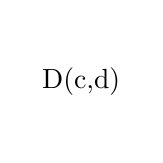
\begin{tikzpicture}[every node/.style={circle, minimum size=8mm}, level/.style={sibling distance=40mm/#1}, level distance=20mm]
                \node {D(c,d)};
            \end{tikzpicture}

            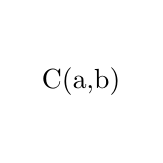
\begin{tikzpicture}[every node/.style={circle, minimum size=8mm}, level/.style={sibling distance=40mm/#1}, level distance=20mm]
                \node {C(a,b)};
            \end{tikzpicture}

            \begin{tikzpicture}[every node/.style={circle, minimum size=8mm}, level/.style={sibling distance=40mm/#1}, level distance=20mm]
                \node {B(a, b, c, d)}
                    child {node {C(a,b)}}
                    child {node {D(c,d)}};
            \end{tikzpicture}

            \begin{tikzpicture}[every node/.style={circle, minimum size=8mm}, level/.style={sibling distance=40mm/#1}, level distance=25mm]
                \node {A(b, d)}
                    child {node {B(a, b, c, d)}
                    child {node {C(a,b)}}
                    child {node {D(c,d)}}};
                    
            \end{tikzpicture}

            The proof tree for $A(b,d)$ already contains proofs for all the other elements of the program so that it would be enough to check this single tree.
        \end{example}

        We can define an element member function for trees in the usual way:

        \begin{lstlisting}
            def elementMember (a: A) (t: tree A): Bool  :=
            match t with
            | tree.node a' l => (a=a') ∨
             List.any l.attach (fun ⟨x, _h⟩ => elementMember a x)
        \end{lstlisting}
        In order for a tree to be valid all subtrees must be valid. A ground atom $ga$ is exactly then a member of a tree $t$ if there is a subtree of $t$ of which $ga$ is the root, so that if a proof tree is valid all elements are a subset of the semantics.

        \begin{lstlisting}
            lemma allTreeElementsOfValidTreeInSemantics 
            (t: proofTree τ)  (P: program τ) (d: database τ) 
            (valid: isValid P d t)(ga:groundAtom τ)(mem: elementMember ga t):
             ga ∈ proofTheoreticSemantics P d :=
        \end{lstlisting}

        This allows us to establish the alternative property of \texttt{validateTreeList}

        \begin{lstlisting}
            lemma validateTreeListUnitIffSubsetSemanticsAndAllElementsHaveValidTrees 
            (P: List (rule τ)) (d: database τ) (l: List (proofTree τ)) 
            (ruleToString: rule τ → String) : validateTreeList P d l  ruleToString = Except.ok () ↔
            {ga: groundAtom τ| ∃ (t: proofTree τ), t ∈ l ∧ elementMember ga t } ⊆ proofTheoreticSemantics P.toFinset d 
            ∧ ∀ (t: proofTree τ), t ∈ l → isValid P.toFinset d t
        \end{lstlisting}

        Now it is enough to pass just one proof tree from our example to validate the whole input and use in general less trees. 

        \subsection{Graph validation}

        We have finished the last section with a method to check whether a result is a subset of the semantics. For this we need a list of trees representing the result set. Finding such a list is however difficult. Viewing a tree as a set of its elements we see that it is an instance of the NP-hard set cover problem. Additionally, we found in practice that the datalog reasoner we used did only return a list of derivations. Constructing trees from this turned out to be computationally expensive, but the output can be interpreted as a directly acyclic graph. In the following section we describe how to validate such a graph.

        A number of different results of graph theory are already proven in mathlib. Nonetheless, we defined our own graph model in Lean for this section due to two main reasons. Firstly, the graph defined in mathlib is a undirected graph, but we require a directed graph so that we can see for a vertex (which represents a ground atom) which neighbors were used to derive it and which neighbors were derived from it. Secondly, the graph represents the edge relation as a map to \texttt{Prop} which is in general not computable.


        Our graph model consists of a list of vertices and a function that maps to each element the list of its predecessors. Representing the vertices as a list allows us to iterate over all vertices when validating the graph. We used a function to the predecessors instead of a adjancency matrix similar to the definition in mathlib in order to directly get the predecessors to a node instead of having the iterate over all vertices and check the adjancency matrix. This approach does have a small drawback. Suppose we want to determine whether a property holds for every vertex and do this by exploring the graph using depth-first search and we find a counterexample by following the predecessors. Nothing states that this vertex is actually in the graph, i.e. the list of vertices. This is an undesireable property so that we additionally ask for a proof that the predecessors of every vertex are again vertices in the graph.

        \begin{lstlisting}
            structure Graph (A: Type) where
                (vertices: List A)
                (predecessors: A → List A)
                (complete: ∀ (a:A), a ∈ vertices →  
                ∀ (a':A), a' ∈ predecessors a → a' ∈ vertices)
        \end{lstlisting}
        
        A standard definition of graph theory are walks as a sequence of connected edges. As we do not have edges directly, we represent this as a list of elements with two properties. A list of elements is a walk in a graph, if all elements are a vertices of the graphs and neighboring vertices are connected via the the predecessor relation of the graph. Due to the completeness property of the graph it would also be sufficient to express that the last element of the path is in the graph. 

        \begin{lstlisting}
            def isWalk (l: List A) (G: Graph A): Prop :=
            ( ∀ (a:A), a ∈ l → a ∈ G.vertices ) 
            ∧ ∀ (i: ℕ), i > 0 → ∀ (g: i < l.length), 
            l.get (Fin.mk i.pred (pred_lt i l.length g)) ∈ 
             G.predecessors (l.get (Fin.mk i g) )
        \end{lstlisting}

        We note that we do allow empty paths. This simplifies some proofs and algorithms even if there is no direct equivalent in graph theory. We specifically use lists as we are going to expand walks at the front when exploring the graph.  
        
        \begin{lemma}
            Let $w$ be a walk in a graph $G$ of the form $a::tl$. Then also $b::a::tl$ is a walk in $G$ for every predecessor $b$ of $a$.
        \end{lemma}

        Using walks we can define cycles. Every cycle is a walk. Additionally we require that it the start and the end of the walk are equal. In order to have a start and end we have to exclude the empty walks. Additionally, we exclude walks of a single element. Allowing them as cycles would mean that there are no acyclic graphs.

        \begin{lstlisting}
            def isCycle (l: List A) (G: Graph A): Prop :=
            if h: l.length < 2
            then False
            else
                have l_not_zero: 0 < l.length :=
                by
                cases ll: l.length with
                | zero =>
                    rw [ll] at h
                    simp at h
                | succ n =>
                    simp

                isWalk l G ∧
                 l.get (Fin.mk 0 l_not_zero) 
                 = l.get (Fin.mk l.length.pred (Nat.pred_lt (Ne.symm (Nat.ne_of_lt l_not_zero))))
        \end{lstlisting}

        A graph is then acyclic if no list represents a cycle in it.

        \begin{lstlisting}
            def isAcyclic (G: Graph A) := ∀ (l: List A), ¬ isCycle l G
        \end{lstlisting}

        We need to check whether a given graph is acyclic as only those graphs represent valid derivations. A cycle would mean that we used an atom to derivate itself and we could not get a valid proof tree for this element. We are going to use depth-first search to check whether a graph is acyclic. For this we need an alternative characterization of acyclicity.
        A first candidate for this would be the membership in a cycle.

        \begin{lemma}
            A graph is acyclic iff no vertice is a member in a cycle.
        \end{lemma}

        Ideally, we want this characterization to be an iff connection between a vertice and its predecessors. Unfortunately the statement does not hold for this characterization.

        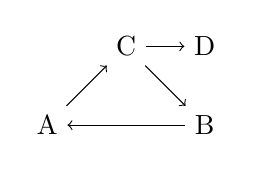
\begin{tikzpicture}
            \node (A) at (0,0) {A};
            \node (B) at (2,0) {B};
            \node (C) at (1,1) {C};
            \node (D) at (2,1) {D};
        
            \draw[->] (B) -- (A);
            \draw[->] (C) -- (B);
            \draw[->] (A) -- (C);
            \draw[->] (C) -- (D);
        \end{tikzpicture}

        D is not a member in a cycle, but its predecessor C is, so that an iff does not hold. Instead we see that D can be reached from a cycle using some walk. If it can be reached from a cycle, then also one of its predecessors can be reached from a cycle. We are going to formalize this idea in the following lemmas.

        Let $a$ and $b$ be two nodes. We say that $a$ can reach $b$ in $G$ if there exists a walk in $G$ that starts with $a$ and ends with $b$.

        \begin{lstlisting}
            def canReach (a b: A) (G: Graph A):= ∃ (w: List A) (neq: w ≠ []),
            isWalk w G ∧
            w.get (Fin.mk 0 (getFirstForNonequal_isLt w neq)) = a ∧
            w.get (Fin.mk w.length.pred (getLastForNonequal_isLt w neq)) = b
        \end{lstlisting}

        A singleton path allows us to show that any element can reach it self. Additionally, if $a$ can reach $b$ and $b$ is a predecessor of $c$ we can extend the path from $a$ to $b$ with $c$ in order to demonstrate that $a$ can reach $c$. Using the \texttt{canReach} predicate we can now express a different characterization for acyclicity, being reachable from a cycle. A node $a$ is reachable from a cycle $c$, if there exists a node $b$ in the cycle that reaches $a$. In the previous example $D$ is reached from a cycle as $C$ is in a cycle and $C$ reaches $D$. The same holds for $C$ as $C$ reaches itself.

        \begin{lstlisting}
            def reachedFromCycle (a:A) (G: Graph A):=
             ∃ (c: List A), isCycle c G ∧ ∃ (b: A), b ∈ c ∧ canReach b a G
        \end{lstlisting}

        \begin{lemma}
            A graph $G$ is acyclic iff all vertices of $G$ are not reached from a cycle.
        \end{lemma}
        \begin{proof}
            If $G$ is acyclic, then showing that all vertices of $G$ are not reached from a cycle is equivalent to showing that any cycle in $G$ cannot reach any element. Due to the acyclicity we know that no cycles exist in G so that the first direction is shown.

            The back direction is proved via contradiction. Assuming that the graph is not acyclic, we know that there must exist a cycle $c$ in $G$. Cycles in $G$ are nonempty lists of vertices that are all in $G$. As any vertex can reach itself, there are vertices that are reached from a cycle in contrast to our assumption, so that we have reached the contradiction.
        \end{proof}

        \begin{lemma}
            A node $a$ is not reached from a cycle iff all predecessors $b$ are not reached from a cycle.
        \end{lemma}
        \begin{proof}
            Both directions are proven via contradiction. For the first we have that there is a predecessor $b$ of $a$ that is reached from a cycle. Then we can simply extend the path by adding $a$ and then $a$ would be reached from a cycle.

            For the backdirection we assume that $a$ is reached from a cycle and try to show then one of its predecessors must also be reached from a cycle. 
            If $a$ is reached from a cycle $c$ with an element $b$ we consider two cases. 
            If $b$ would be a predecessor, then we have reached a contradiction as $b$ is in the circle and reaches itself. Now we assume that $b$ is not a predecessor of $a$. Again we can consider two cases. If the path is of length one then $a$ and $b$ must be equal and $a$ is a member in a cycle. As long as $a$ is not the first element in the cycle, we can simply pick the preceeding element in the cycle due to the connectness property of the walk. This does not work if $a$ is the first element, but since it is a cycle $a$ must also be the last element and we can pick the predecessor of the last element, which is a predecessor of $a$ and in a cycle.

            If $a$ is reached from a path longer than length 1, we simply pick the subpath without the last element. This is not empty and ends with a predecessor of $a$, which is therefore reached by a cycle. In every case we reached a contradiction so that the claim must be true.
        \end{proof}

        This completes a characterization of acyclicity that has an iff relation between a node and its predecessors. We still need a method to detect a cycle. We are going to explore the graph via walks and add the current element to the walk whenever we reach a new node. If we see a node again, we have reached a cycle.

        \begin{lemma}
            Let $w$ be a walk in a graph $G$ and $a$ be a node of $G$ so that $a::w$ is also a walk in $G$. If $a$ is a member of $w$, then there exists a cycle in $G$.
        \end{lemma}

        For this we need to extract the walk from $a$ to $a$ out of $a::w$. This is done by the \texttt{getSubListToMember} function. We are given an element $a$, a list $l$ and a proof of $a\in l$ and want to return the sub list until $a$. This is defined inductively. The empty case of $l$ is impossible as $a$ can be a member of the empty list. In the cons case we keep the head element of the list in the result. If this is already $a$, then we stop, else $a$ must be a member in the tail and we continue.

        \begin{lstlisting}
            def getSubListToMember (l: List A) (a: A) (mem: a ∈ l): List A :=
            match l with
            | [] =>
                have h: False :=
                by
                simp at mem

                False.elim h
            | hd::tl =>
                if p: a = hd
                then [hd]
                else
                have mem': a ∈ tl :=
                by
                    simp[p] at mem
                    apply mem
                hd::getSubListToMember tl a mem'
        \end{lstlisting}

        In any case the list is never empty as we return at least the head of the list we called \texttt{getSubListToMember} on and in both cases the resulting list $l'$ starts with the same element as $l$ used to. By calling it on $w$ with the member $a$ the result $l'$ starts with the same element as $w$. Since $a::w$ was a walk, we therefore can also extend $l'$ with $a$ and preserve a walk assuming that $l'$ preserves a walk. This can be proven by induction. If we have reached the element we return a list with a single element that is a member of $G$, which is always a walk. If not we keep the element and add this to the result of \texttt{getSubListToMember} on the tail. This result is by the induction hypothesis a walk and by the previous result keeps the first element so that we can attach $hd$ again to the front and get a walk. Now we now that the result of \texttt{getSubListToMember a w mem} is a walk and that also \texttt{a::(getSubListToMember a w mem)} is walk. 
        In order to show that this a cycle we need two more facts. Firstly, this list should have a length of at least two. This is the case as \texttt{getSubListToMember} never returns an empty list, so that it has at least length one and also attaching $a$ to the front increases the length by one. Secondly, we need the resulting list of \texttt{getSubListToMember a w mem} to end with $a$ so that \texttt{a::(getSubListToMember a w mem)} is cycle. This can again be proven by induction, since the list only ends when $a$ is encountered. 



    \section{Completeness}

    In the previous chapter we described a method why an atom is in the datalog semantics. This criteria is however not sufficient to recognize a solution. The empty list passes this test for any program while not being the semantics in most cases. Proof trees were a method to recognize why a ground atom is part of the semantics, but we are not aware of any simple way to describe why a ground atom is not in the semantics. Instead we want to show that the set of elements in the proof trees, $S$ are complete in the sense that nothing else can derived from it any more. This is the case when the $T_P$ operator has a fixed-point for $S$ or alternatively when $S$ is a model. In this chapter we are going to create a certified model checker to show the completeness. If $S$ passed the tree validation algorithm and is a model the following statements hold:

    \[ S \subseteq \mathtt{proofTheoreticSemantics\ P\ d} = \mathtt{modelTheoreticSemantics\ P\ d} \subseteq S \]

    \subsection{Partial ground rules}
    
        We defined the model property on the ground program $ground(P)$. In order to check if a set of ground atoms is a model for a program we therefore have to ground the program. We want to avoid simply grounding all the rules at once and instead do it in a more intelligent way. For this we introduce a new data structure, the partial ground rule. This bears some similarities to the rules we defined in chapter 3. It has a head that is an atom. The body is split into two lists. The first list contains the ground atoms and represents the atoms in the rule we already grounded, whereas the second list consists of the so far ungrounded atoms in the rule body. We want to move the ungrounded atoms one by one into the grounded list by applying substitutions, which map all variables of this atom to constants, so that we can transform this atom into a ground atom.

        \begin{lstlisting}
            structure partialGroundRule (τ: signature)  where
                head: atom τ
                groundedBody: List (groundAtom τ)
                ungroundedBody: List (atom τ)
        \end{lstlisting}

        \begin{example}
            A rule $r := q(X) :- r(a, b), t(X, c), s(c, d), u(d, X) .$ may be viewed as the following partial ground rule
            $pgr_1 = $
            \begin{lstlisting}
                {
                    head:= q(X),
                    groundedBody := [],
                    ungroundedBody := [r(a, b), t(X, c), s(c, d), u(d, X)]
                }
            \end{lstlisting}
            
            This representation does not look any different to the rule itself as we do not use the grounded body at all. We can however move ground atoms from the ungrounded body into the grounded body. The order of the atoms in the body does not matter semantically as we use a set definition when defining the criteria for a rule being true, so that we can simply move all ground atoms in the grounded body.

            \begin{lstlisting}
                {
                    head:= q(X),
                    groundedBody := [r(a, b), s(c, d)],
                    ungroundedBody := [t(X, c),  u(d, X)]
                }
            \end{lstlisting}

        \end{example}

        We can transform any rule into a partial ground rule by setting the head as the head, the body as the ungrounded body and setting the grounded body to be empty.

        \begin{lstlisting}
            def partialGroundRuleFromRule (r: rule τ): partialGroundRule τ :=
            {
                head := r.head, 
                groundedBody := [],
                ungroundedBody := r.body
            }
        \end{lstlisting}

        \begin{example}
            $pgr_1$ is exactly the result of \texttt{partialGroundRuleFromRule $r$}.
        \end{example}

        We choose this representation instead of the approach used for $pgr_2$ as this does not require iterating over the whole body to find ground atoms. As we will apply multiple substitutions in the grounding process, we will create anyways ground atoms in different place to the atom in the body we are currently trying to ground.

        Any partial ground rule can also be transformed back into a rule by concatenating the grounded and ungrounded body and combining creating first a partial ground rule from a rule and then transforming the resulting partial ground rule yields the original rule. This does not hold if we swap the operations as we do not explicitly move atoms without variables from the start of the body into the grounded body.

        \begin{lstlisting}
            def partialGroundRule.toRule (pgr: partialGroundRule τ)
            : rule τ :=
    
            {
                head:= pgr.head, 
                body := (List.map (groundAtom.toAtom) pgr.groundedBody)
                ++ pgr.ungroundedBody
            }

            lemma partialGroundRuleToRuleInverseToFromRule (r: rule τ): 
                r = partialGroundRule.toRule (partialGroundRuleFromRule r)
        \end{lstlisting}

        \begin{example}
            The application of \texttt{partialGroundRule.toRule} on $pgr_1$ yields $r$ as predicted by the lemma.

            If we swap both functions and first apply \texttt{partialGroundRule.toRule} to a partial ground rule and then convert the resulting rule back to a partial ground rule, we see that this is no longer equal. Applying {partialGroundRule.toRule} to $pgr_2$ results in the rule $ q(X) :- r(a, b), s(c, d), t(X, c),  u(d, X) . $. Converting this back into a partial ground rule with \texttt{partialGroundRuleFromRule} we gain 

            \begin{lstlisting}
                {
                    head:= q(X),
                    groundedBody := [],
                    ungroundedBody := [r(a, b), s(c, d), t(X, c),  u(d, X)]
                }
            \end{lstlisting}
            which is different from $pgr_2$
        \end{example}

        Using the transformation to rules we can lift defintions like safety or being true to partial ground rules.

        \begin{lstlisting}
            def partialGroundRule.isSafe (pgr: partialGroundRule τ) :=
                pgr.toRule.isSafe

            def partialGroundRule.ruleTrue (pgr: partialGroundRule τ) 
            (i: interpretation τ) :=
                ruleTrue pgr.toRule i
        \end{lstlisting}

        So far we only split the body into two parts and have the goal of applying substitutions to move everything into the grounded body. This is not to different to just applying groundings directly. 
        This process allows us to potentially stop early. If the substitutions we applied so far resulted in a ground atom that is not part of the interpretation $i$ we already know that the rule is true. No matter how the remaining variables are mapped, the body will never be a part of $i$ and therefore the antecedent is false and the rule is therefore true. We call a partial ground rule \textit{active in an interpretation} $i$ where all ground atoms in the \texttt{groundedBody} 

        \begin{lstlisting}
            def active (pgr: partialGroundRule τ) (i: interpretation τ):=
            ∀ (ga: groundAtom τ), ga ∈ pgr.groundedBody → ga ∈ i 
        \end{lstlisting}

    \subsection{Explore grounding}

    \bibliography{main.bib}
    \bibliographystyle{plain}
\end{document}